\chapter{Capa de Negocio}
\section{Introducción}

Esta capa consiste en entender los conceptos que definen la estructura estática de la organización en términos de las entidades que componen la organización y las interacciones presentadas entre estas. Entidades como actores de negocio, roles de negocio, funciones de negocio, etc, que se comportan por medio de un diseño orientado al servicio, es decir, las funciones o procesos de negocio interno y externo de la organización como las responsabilidades \cite{BolanosCastro2019}.

Por otra parte, es importante resaltar que, dentro de la arquitectura de negocio se tiene que la relación entre entidades como se menciona anteriormente, de forma externa e interna, determina un proceso de comunicación entre estas, contando con interfaces que permiten el acceso a diferentes servicios mediante colaboraciones dadas por las entidades organizacionales \cite{BolanosCastro2019}.

A continuación se presentan cada uno de los puntos de vista de la capa de negocio  a partir del soporte realizado por el Área de Investigación de Análisis de datos a los investigadores de la Subdirección de Investigaciones, otras Subdirecciones y demás unidades funcionales del Instituto  de Cancerología.

%-------------Punto de Vista de la Organización----------%
\newpage
\section{Punto de Vista de la Organización}
El Punto de Vista de Organización se centra en la organización interna de una empresa, un departamento, una red de empresas o de otra entidad organizativa. Se utiliza para identificar las competencias, la autoridad y las responsabilidades en una organización\cite{BolanosCastro2019}.

En la Figura \ref{PvOrganizacion}, se plantea el Caso para el Punto de Vista de Organización con cada uno de los elementos que interactúan entre sí. 

\begin{figure}[h!]
	\centering
	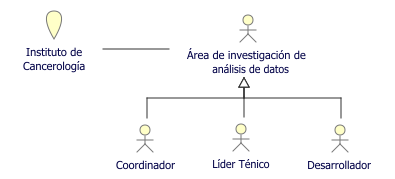
\includegraphics[width=1\linewidth]{ARQUITECTURA/imgs/CapaNegocio/1_PvOrganizacion}
	\caption{Punto de Vista de la Organización}
	\label{PvOrganizacion}
\end{figure}

\begin{enumerate}[label=\textbf{\arabic*})]
\item  \textbf{\textbf{Instituto  de Cancerología}:} Este elemento hace referencia a la localización geográfica donde se encuentra ubicada  la organización. El instituto de  Cancerología cuenta con siete grupos de investigación que desarrollan diversas actividades según su campo de acción: investigación clínica, investigación epidemológica, biología del cáncer e investigación en el área de la salud pública.Esta localización está asociada al actor \textit{Área de investigación de análisis de datos}.


\item \textbf{Área de Investigación de análisis de datos:} Corresponde a una de las dependencias del área de investigación la cual  tiene por objetivo dar soporte a los investigadores de la Subdirección de Investigaciones, otras Subdirecciones y demás unidades funcionales del Instituto  de Cancerología, haciendo uso de métodos computacionales para el manejo y análisis de datos Oncológicos. Este actor tiene como \textit{especialización} tres actores los cuales se muestran a continuación:
\newpage
\begin{itemize}
    \item  \textbf{\textit{Coordinador:}}
	Es la persona encargada de regular, gestionar, dirigir y supervisar el Área de Investigación de análisis de datos de Oncología para que el soporte realizado a los investigadores de la Subdirección de Investigaciones, otras Subdirecciones y demás unidades funcionales se realice correctamente.
	
	\item  \textbf{\textit{Líder Técnico:}}
	Es la persona con conocimiento técnico avanzado en los temas de análisis de datos de Oncología y es el  responsable de asignar y definir las  tareas y el tiempo necesario en el desarrollo e implementación de los recursos  según las necesidades presentadas por los investigadores y las unidades funcionales del Instituto  de Cancerología.
	\item  \textbf{\textit{Desarrollador:}}
	Es la persona encargada de cumplir con las implementaciones presentadas en el ámbito de análisis de datos de Oncología y que da  solución a cada uno de los requerimientos y necesidades presentadas por los  investigadores y las unidades funcionales del Instituto  de Cancerología.
	
\end{itemize}

\end{enumerate}

%-------------Punto de Vista de Cooperación de Actor---------%
\newpage
\section{Punto de Vista de Cooperación de Actor}
El Punto de Vista de Cooperación de Actor se centra en las relaciones de los actores entre sí y su entorno. Se utiliza para determinar las dependencias externas y colaboraciones, y muestra la cadena de valor o la red en la que actúa el actor\cite{BolanosCastro2019}.

En la Figura \ref{PvCooperacionActor}, se plantea el Caso para el Punto de Vista de cooperación de Actor donde se describen los elementos que interactúan este punto de vista.

\begin{figure}[h!]
	\centering
	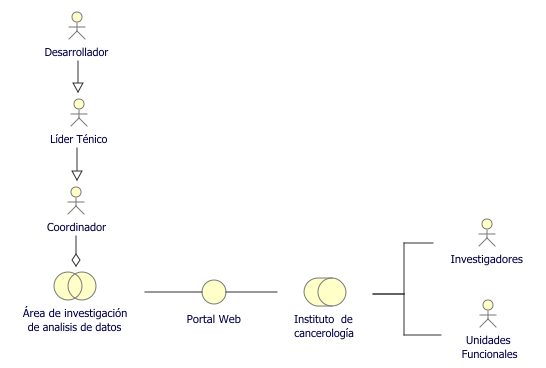
\includegraphics[width=1\linewidth]{ARQUITECTURA/imgs/CapaNegocio/2_PvCooperacionActor}
	\caption{Punto de Vista de Cooperación de Actor}
	\label{PvCooperacionActor}
\end{figure}

\begin{enumerate}[label=\textbf{\arabic*})]
\item  \textbf{Portal Web :} Es el medio de comunicación entre el Área de Investigación de análisis de datos  y los investigadores de la Subdirección de Investigaciones, otras Subdirecciones y demás unidades funcionales del Instituto  de Cancerología. Esta interfaz tiene una asociación con el rol del  \textit{Área de Investigación de análisis de datos}  y es usada por el rol \textit{Instituto  de Cancerología}.

\newpage
\item  \textbf{Instituto  de Cancerología:} A el rol  instituto de  de cancerología están asociados el actor \textit{Investigador } y el actor \textit{Unidades funcionales }. Estos roles se describen a continuación: 
\begin{itemize}
\item  \textbf{\textit{Investigadores :}}  Este rol está conformado por todos los grupos de investigación en cáncer del país registrados ante Colciencias y adicionalmente, con representantes de diferentes tipos de usuarios del conocimiento generado por la investigación como son las sociedades médicas, los prestadores de servicios oncológicos, los aseguradores, las autoridades sanitarias y los pacientes entre otros. 

\item  \textbf{\textit{Unidades Funcionales :}}  Este rol está conformado por las unidades clínicas ubicadas al interior del Instituto  de Cancerología cuya función es evaluar la situación de salud del paciente con diagnóstico presuntivo de cáncer. 
\end{itemize}
\end{enumerate}

%-------------Punto de Vista de Cooperación de Actor------------------------%
\newpage
\section{Punto de Vista de la Función de Negocio}
El Punto de Vista de la Función de Negocio muestra las principales funciones de negocio de una organización y sus relaciones en términos de los flujos de información, valor o bienes entre
ellos.

Adicionalmente, proporciona una visión de alto nivel de las operaciones generales de la empresa y puede utilizarse para identificar las competencias necesarias o estructurar una organización de acuerdo con sus principales actividades
\cite{BolanosCastro2019}.

En la Figura \ref{PvFuncion}, se plantea el Caso para el Punto de Vista de Función de Negocio donde se describen los elementos que interactúan en este punto de vista.

\begin{figure}[h!]
	\centering
	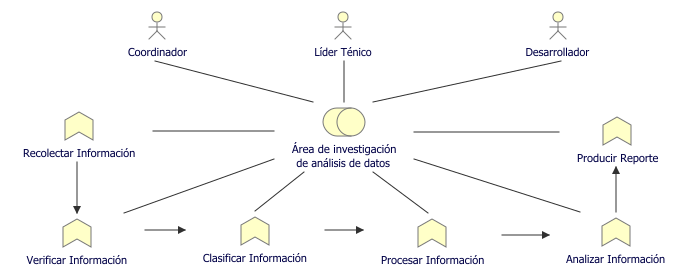
\includegraphics[width=1\linewidth]{ARQUITECTURA/imgs/CapaNegocio/3_PvFuncion}
	\caption{Punto de Vista de la Función del negocio}
	\label{PvFuncion}
\end{figure}

\begin{enumerate}[label=\textbf{\arabic*})]
\item  \textbf{Área de Investigación de análisis de datos:} Este rol corresponde  a una de las dependencias del área de investigación la cual  tiene por objetivo dar soporte a los investigadores de la Subdirección de Investigaciones, otras Subdirecciones y demás unidades funcionales del Instituto  de Cancerología. Este rol está asociado a los actores coordinador, líder técnico y desarrollador y a seis diferentes funciones las cuales se muestran a continuación:
\newpage
\begin{itemize}
\item  \textbf{\textit{Recolectar Datos:}} Esta función se encarga de recopilar y medir la información de los Data Set que contienen variables oncológicas específicas que requieren ser analizadas.

\item  \textbf{\textit{Verificar Datos:}}  Esta función se basa en la identificación  y corrección o eliminación de registros de datos erróneos encontrados en los Data Set oncológicos. Este proceso permite encontrar datos incompletos, incorrectos, inexactos, no pertinentes, etc. y luego substituir, modificar o eliminar para realizar posteriormente la clasificación de los mismos.

\item  \textbf{\textit{Clasificar Datos:}} Esta función se basa en la distribución por medio de algoritmos de Machine Learning de los Data Set que contienen variables oncológicas específicas que al ser comparados con trazas características de casos de cáncer avanzados permiten agruparlos en diferentes categorías según el porcentaje de padecimiento del mismo.

\item  \textbf{\textit{Procesar Datos:}} Esta función se basa en la manipulación de los Data Set oncológicos  para generar información por medio de gráficos y estadísticas haciendo uso de los modelos de Machine Learning.

\item  \textbf{\textit{Analizar Datos:}} Esta función se encarga de examinar los Data Set que dieron como resultado de las funciones anteriores y los gráficos obtenidos con el propósito de sacar conclusiones diagnosticas sobre el posible padecimiento de cáncer.

\item  \textbf{\textit{Generar Reportes:}} Esta función se encarga de crear en un módulo informativo los datos relevantes obtenidos de los Data Set oncológicos solicitados para ser analizados por medio de tablas, estadísticas y gráficos que dan el resumen de los resultados, conclusiones y diagnósticos sobre el posible padecimiento de cáncer en el individuo.
\end{itemize}
\end{enumerate}

%-------------Punto de Vista de Proceso de Negocio------------------------%
\newpage
\section{Punto de Vista de Proceso de Negocio}
El Punto de Vista de Proceso de Negocio se utiliza para mostrar la estructura y composición de alto nivel de uno o más procesos empresariales\cite{BolanosCastro2019}.

Junto a los procesos mismos, este punto de vista contiene otros conceptos directamente relacionados, tales como: los servicios que un proceso de negocio ofrece de manera global, mostrando como un proceso contribuye a la realización de los productos de la empresa; la asignación de los procesos de negocio a las funciones, lo que da una idea de las responsabilidades de los actores asociados; la información utilizada por el proceso de negocio. Cada uno de estos puede ser considerado como una sub-vista de la vista del proceso empresarial\cite{BolanosCastro2019}.

En la Figura \ref{PvProceso}, se plantea el Caso para el Punto de Vista de Proceso de Negocio aplicado al Área de Investigación de análisis de datos. A continuación, se describen los elementos que interactúan en este punto de vista.

\begin{figure}[h!]
	\centering
	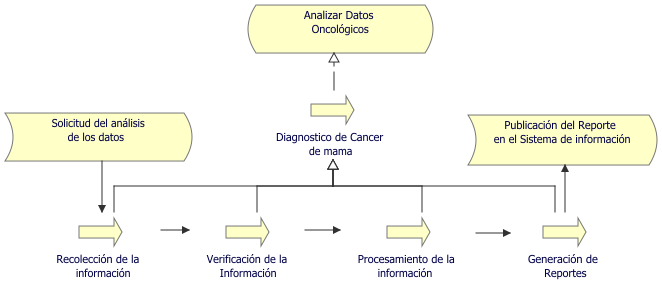
\includegraphics[width=1\linewidth]{ARQUITECTURA/imgs/CapaNegocio/4_PvProceso}
	\caption{Punto de Vista del proceso del negocio}
	\label{PvProceso}
\end{figure}

\begin{enumerate}[label=\textbf{\arabic*})]
	\item  \textbf{Analizar Datos Oncológicos:} Este servicio realiza el análisis de los datos entregados por  los investigadores de la Subdirección de Investigaciones, otras Subdirecciones y demás unidades funcionales del Instituto  de Cancerología para generar diagnósticos oncológicos. Es brindando por el proceso de  \textit{Análisis de Datos}.
	\newpage
	\item  \textbf{Diagnostico de Cáncer de mama:} El proceso de Diágnostico de Cáncer de mama es fundamental debido que cumple con el objetivo principal de facilitar el análisis de datos oncológicos a las diferentes áreas y unidades funcionales de la organización. Además, este proceso está conformado de otros procesos en secuencia que dan solución al servicio final.

	\item  \textbf{Solicitud de análisis de datos:} Este evento es el que origina los sub-procesos para lograr el objetivo del servicio principal. Este corresponde a la acción en donde  los investigadores de la Subdirección de Investigaciones, otras Subdirecciones y demás unidades funcionales del Instituto  de Cancerología desean que se analicen diferentes Data Set oncológicos para obtener un reporte. Está relacionado  directamente con el sub-proceso de \textit{Recolección de información}  que es el primer proceso para analizar los datos solicitados.
	
	\item  \textbf{Recolección de información:} Este sub-proceso se encarga de recopilar y organizar toda la información que contiene datos oncológicos de cada paciente que son necesarios para su posterior verificación. Es el primer subproceso llevado a cabo para el objetivo de análisis de datos oncológicos que a su vez, desencadena un nuevo subproceso mediante una relación causal.
	
	\item  \textbf{Verificación de la información:} Este sub-proceso se encarga de identificar si las variables oncológicas solicitadas están completas. Además, si la información entregada esta completa pero algunos de los datos se encuentran erróneos o defectuosos se sustituyen para realizar posteriormente la clasificación de los mismos. Este sub-proceso desencadena un nuevo subproceso mediante una relación causal.
	
	\item  \textbf{Procesamiento de la información:} Este sub-proceso se encarga de usar los datos oncológicos  verificados para generar información relevante por medio de gráficos y estadísticas. Este sub-proceso desencadena un nuevo subproceso mediante una relación causal.
	
	\item  \textbf{Generación  de Reportes:} Este sub-proceso se encarga de organizar en un módulo la información de los resultados obtenidos de los Data Set oncológicos solicitados para ser analizados por medio de tablas, estadísticas y gráficos. Este sub-proceso desencadena un nuevo subproceso mediante una relación causal.
	\newpage
	\item  \textbf{Publicación del Reporte en el portal web :} Este evento es el que finaliza el flujo conformado por los sub-procesos anteriores y representa la acción de difundir la información oncológica analizada y  los resultados diagnósticos obtenidos en el Portal web  de cada uno de los datos solicitados para análisis. Este evento es accionado por el sub-proceso \textit{Generación  de Reportes}.
\end{enumerate}

%-------------Punto de Vista de Cooperación de Proceso de Negocio}o------------------------%
\newpage
\section{Punto de Vista de Cooperación de Proceso de Negocio}
El Punto de Vista de Cooperación de Proceso de Negocio se utiliza para mostrar las relaciones de uno o más procesos de negocio entre si y/o con su entorno\cite{BolanosCastro2019}.

Puede utilizarse tanto para crear un diseño de alto nivel de procesos empresariales dentro de su contexto, como para proporcionar un gestor operativo responsable de uno o más de dichos procesos con información sobre sus dependencias \cite{BolanosCastro2019}.

En la Figura \ref{PvCooperacionProces}, se plantea el Caso para el Punto de Vista de Cooperación de Proceso de Negocio aplicado al Área de Investigación de análisis de datos. A continuación, se describen los elementos que interactúan en el punto de vista.

\begin{figure}[h!]
	\centering
	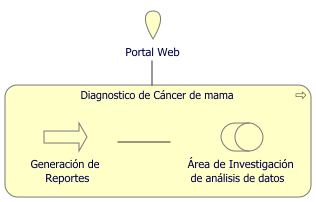
\includegraphics[width=0.75\linewidth]{ARQUITECTURA/imgs/CapaNegocio/5_PvCooperacionProceso}
	\caption{Punto de Vista de Cooperación de Proceso de Negocio}
	\label{PvCooperacionProces}
\end{figure}

\begin{enumerate}[label=\textbf{\arabic*})]
\item  \textbf{Portal Web :} Es el medio de comunicación entre el Área de Investigación de análisis de datos  y los investigadores de la Subdirección de Investigaciones, otras Subdirecciones y demás unidades funcionales del Instituto  de cancerología. Está relacionado directamente con el servicio de \textit{Diagnostico de Cáncer de mama}. 

\item  \textbf{Diagnóstico de Cáncer de mama:} Este servicio cumple el objetivo dar soporte a los investigadores de la Subdirección de Investigaciones, otras Subdirecciones y demás unidades funcionales del Instituto  de Cancerología con respecto al análisis de datos oncológicos.  Es brindado por el proceso de \textit{Análisis de Datos}.
\newpage
\item  \textbf{Generación  de Reportes:} Este sub-proceso hace referencia a la organización de la información de los resultados obtenidos de los Data Set oncológicos solicitados para ser analizados por medio de tablas, estadísticas y gráficos.

\item \textbf{Área de Investigación de análisis de datos:} Corresponde área de investigación la cual da soporte a los investigadores de la Subdirección de Investigaciones, otras Subdirecciones y demás unidades funcionales del Instituto  de Cancerología por medio reportes generados con base a los datos solicitados.

\end{enumerate}

%-------------Punto de Vista de Producto-----------------------------%
\newpage
\section{Punto de Vista de Producto}
El Punto de Vista de Producto representa el valor que estos productos ofrecen a los clientes u otras partes externas involucradas\cite{BolanosCastro2019}.

Adicionalmente, muestra la composición de uno o más productos en términos de los servicios constitutivos-comerciales o de aplicación, y los contratos asociados u otros acuerdos. También se puede utilizar para mostrar las interfaces a través de las cuales se ofrece este producto, y los eventos asociados al mismo\cite{BolanosCastro2019}.

En la Figura \ref{PvProducto}, se plantea el Caso para el Punto de Vista de Producto.A continuación, se describen los elementos que interactúan en el punto de vista.

\begin{figure}[h!]
	\centering
	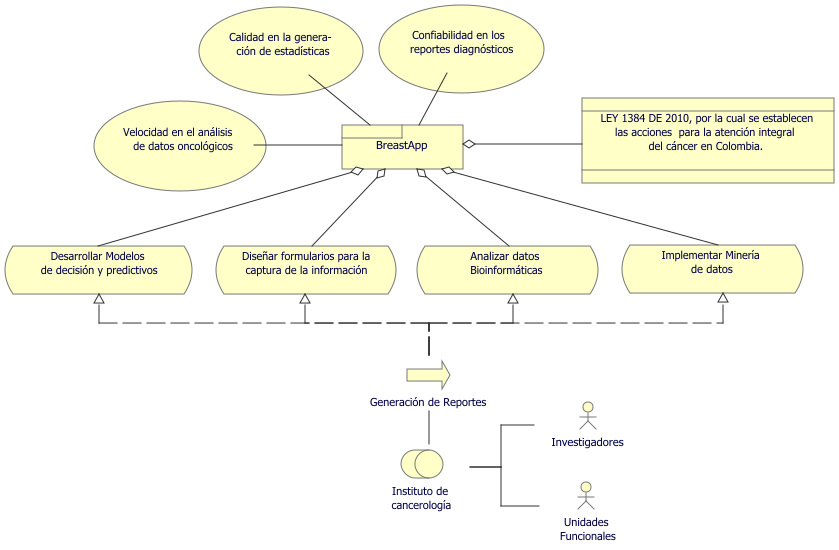
\includegraphics[width=1\linewidth]{ARQUITECTURA/imgs/CapaNegocio/6_PvProducto}
	\caption{Punto de Vista de Producto}
	\label{PvProducto}
\end{figure}

\begin{enumerate}[label=\textbf{\arabic*})]
	
	\item  \textbf{BreastApp:} Este producto corresponde a la generación de reportes diagnósticos según el análisis de datos oncológicos elaborados por los investigadores de la Subdirección de Investigaciones, otras Subdirecciones y demás unidades funcionales del Instituto  de Cancerología. Está compuesto de los siguientes servicios:
	
\begin{itemize}
	\item  \textbf{\textit{Desarrollar Modelos de Decisión y predictivos:}} Este servicio corresponde al uso de modelos de Machine Learning para  para diagnosticar  el padecimiento de cáncer .Este servicio sirve como herramienta para realizar diversas investigaciones y poder  disminuir su tasa de mortandad en Colombia.
	
	\item  \textbf{\textit{Diseñar formularios para la captura de la información:}} Este servicio corresponde a la creación de formularios web de ámbito científico con énfasis en el diagnóstico del cáncer para que los diferentes investigadores y áreas funcionales de la organización proporcionen la información relacionada con los datos de cada individuo.
	
	\item  \textbf{\textit{Analizar Datos Bioinformáticos:}} Este servicio corresponde a los métodos y modelos basados en diferentes sistemas de cómputo numéricos con base a variables del ámbito de la biología para realizar simulaciones que permitan observar el comportamiento de los mismos en diferentes ambientes y determinar una posible solución al problema del padecimiento de cáncer.
	
	\item  \textbf{\textit{Implementar Minería de Datos:}} Este servicio corresponde a la búsqueda de  correlaciones o patrones entre los millones de datos obtenidos de todos los pacientes con cáncer para proporcionar información diagnostica cada vez más específica y exacta de los datos solicitados por los investigadores y las unidades funcionales de la organización.
\end{itemize}
	Ademas, cuenta son los siguientes valores:
\begin{itemize}
		\item  \textbf{\textit{Velocidad en el análisis de datos oncológicos:}} El objetivo principal es realizar de manera eficaz el análisis los datos oncológicos en cuestión para dar una diagnostico  en el menor tiempo posible.
		
		\item  \textbf{\textit{Calidad en la generación de estadísticas:}} El objetivo principal es analizar los datos de una manera profesional   para satisfacer necesidades explícitas de los investigadores y las unidades funcionales de la organización. 
		
		\item  \textbf{\textit{Confiabilidad en los reportes diagnósticos:}} El objetivo principal es generar los reportes oncológicos analizados  con una precisión superior para que la información generada por tablas y gráficos generen un diagnóstico exacto que ayude en las diferentes actividades de los investigadores y las unidades funcionales de la organización.
		
\end{itemize}

	\item  \textbf{Ley 1384 de 2010:} Esta resolución establece las acciones para el control integral del cáncer en la población colombiana, de manera que se reduzca la mortalidad y la morbilidad por cáncer adulto, así como mejorar la calidad de vida de los pacientes oncológicos, a través de la garantía por parte del Estado y de los actores que intervienen en el Sistema General de Seguridad Social en Salud vigente, de la prestación de todos los servicios que se requieran para su prevención, detección temprana, tratamiento integral, rehabilitación y cuidado paliativo.
	
	\item  \textbf{Generación de Reportes:} Implica la organización de la información de los resultados obtenidos en los diagnósticos oncológicos solicitados para ser visualizados por medio de tablas, estadísticas y gráficos. Se asocia con el rol de \textit{Instituto  de cancerología}. A su vez, realiza los servicios descritos anteriormente.
	
	
	\item  \textbf{Instituto  de Cancerología:} Este elemento hace referencia el rol  Instituto de  de cancerología el cual cuenta con siete grupos de investigación que desarrollan diversas actividades según su campo de acción: investigación clínica, investigación epidemiológica, biología del cáncer e investigación en el área de la salud pública. Este rol usa el proceso \textit{Generación de Reporte} y se asigna a los dos actores a continuación:
	
	\begin{itemize}
		\item  \textbf{\textit{Investigadores :}}  Este rol está conformado por todos los grupos de investigación en cáncer del país registrados ante Colciencias y adicionalmente, con representantes de diferentes tipos de usuarios del conocimiento generado por la investigación como son las sociedades médicas, los prestadores de servicios oncológicos, los aseguradores, las autoridades sanitarias y los pacientes entre otros. 
		
		\item  \textbf{\textit{Unidades Funcionales :}}  Este rol está conformado por las unidades clínicas ubicadas al interior del Instituto  de Cancerología cuya función es evaluar la situación de salud del paciente con diagnóstico presuntivo de cáncer. 
	\end{itemize}
	
\end{enumerate}